\documentclass[9pt,twocolumn,twoside]{idsi}
% Defines a new command for the horizontal lines, change thickness here
\newcommand{\HRule}{\rule{\linewidth}{0.5mm}}
% Package for text
\usepackage{textcomp}

\renewcommand{\headrulewidth}{2pt}
\fancypagestyle{plain}{%
  \fancyhead[L]{
    \begin{tabular}{ll}
%        \includegraphics[scale=0.15]{figs/ncsa_vertical}
    \end{tabular}
  }
  \fancyhead[C]{
      	\begin{tabular}[m]{c}
		  	\fontsize{20}{20} Illinois Data Science Initiative
		\end{tabular}
  }

  \fancyhead[R]{
    \begin{tabular}{ll}
%	  	\includegraphics[scale=0.125]{figs/ill}
  	\end{tabular}
  }

  \fancyfoot[C]{\thepage}
}
\pagestyle{plain}
\def \report_title {Processing the Blockchain with Hadoop and Spark}
\author[1,3]{Nishil Shah}
\author[2,3]{Professor Robert J. Brunner}
\affil[1]{National Center For Supercomputing Applications (NCSA)}
\affil[2]{Laboratory for Computation, Data, and Machine Learning}
\affil[3]{Illinois Data Science Initiative}
\title{Processing the Blockchain with Hadoop and Spark}

\begin{abstract}
Using several big data technologies, we process over 100 gigabytes of Bitcoin transactions to yield statistics and trends on the usage of the most popular peer-to-peer electronic currency.
\end{abstract}

\begin{document}

\begin{titlepage}
\center
\textsc{\LARGE Illinois Data Science Initiative}\\[1.5cm]
\textsc{\Large Technical Reports}\\[0.5cm] \HRule \\[0.4cm]
{\huge \bfseries Processing the Blockchain with Hadoop and Spark } \\[0.4cm] \HRule \\[1.5cm]
\Large \emph{Author:}\\ Nishil Shah \\[3cm]
{\large April 11, 2017}\\[3cm] % Date
%\includegraphics{Logo}\\[1cm] % uncomment if you want to place a logo
\vfill
\end{titlepage}
%\include{cover}

\maketitle

\section{Introduction}
\subsection{Bitcoin}
Bitcoin is a peer-to-peer virtual currency built to eliminate the need for intermediaries like businesses and banks who process transactions and handle disputes. Bitcoin accomplishes this with a decentralized system that allows for non-reversible transactions verified by a chain of computational proof, commonly known as the Blockchain. Bitcoin is decentralized in the sense that there is no central authority. The entire ledger of transactions is stored on every node, which carries equal say, in the network. Each node collects incoming transactions into blocks of a limited size. Nodes simultaneously work on a difficult proof-of-work that when found allows the solving node to broadcast the finalized block to other nodes on the network. All other nodes then must verify the block's transactions to ensure its contents are valid before appending it to their local copy of the chain. Anyone can start a Bitcoin node by installing the \href{https://bitcoin.org/en/bitcoin-core/}{Bitcoin Core} software.

There are no tangible "coins". Bitcoins are simply a series of digital messages sent from address to address signed with a private key of the sender. Coins can only be spent from an address if a user has its associated private key. Overall, the Bitcoin system is incredibly robust, allowing for quick and secure transactions without regulation of third-party financial institutions or governments. More information on Bitcoin can be found in the \href{https://bitcoin.org/bitcoin.pdf}{paper} by Bitcoin's creator, \href{https://en.wikipedia.org/wiki/Satoshi_Nakamoto}{Satoshi Nakamoto}.

\subsection{Purpose}
At the time of writing, 1 Bitcoin is equivalent to over 1200 USD; all the Bitcoins in circulation have a market cap of almost 20 billion dollars. Clearly, there is value in Bitcoin as a medium of exchange, store of value, and/or unit of account. A market of such volume is certainly worthy of exploration. Uncovering trends and metrics on the usage of Bitcoins can be useful in predicting future market activity and possibly even help to identify limitations in its underlying system. Technologies like Hadoop and Spark make it simple to model, process, and analyze the immense amount of transactional data in the Bitcoin network.

Overall, the purpose of this technical report is to find patterns in Bitcoin transactions to better understand how people use Bitcoin. Simultaneously we aim to show the procedure involved in applying big data processing to a real world dataset on our Openstack cluster.

\section{Prerequisites}
\subsection{Assumptions}
This technical report assumes:
\begin{itemize}
    \item We have Apache Ambari set up on Openstack as outlined in the technical report, \href{https://github.com/lcdm-uiuc/idsi-core/blob/bitcoin_tr/reports/ambari_openstack_setup/ambari_openstack_setup.pdf}{Setting up Ambari on Openstack Nebula}.
    \item Our Openstack cluster has Hadoop, YARN, and Spark installed.
\end{itemize}
\subsection{Tools}
The following technologies are used in our implementation:
\begin{itemize}
    \item Bitcoin Core v. 0.14.0 [\href{https://bitcoin.org/en/bitcoin-core/}{website}] [\href{https://bitcoin.org/en/download}{download}]
    \item bitcoinj (for parsing) [\href{https://bitcoinj.github.io/}{website}] [\href{https://bitcoinj.github.io/#getting-started}{download}]
    \item Apache\textsuperscript{TM} Hadoop\textsuperscript{\textregistered} [\href{http://hadoop.apache.org}{website}] [\href{http://hadoop.apache.org/#Download+Hadoop}{download}]
    \item Apache Spark\textsuperscript{TM} [\href{http://spark.apache.org/}{website}] [\href{http://spark.apache.org/downloads.html}{download}]
    \item IntelliJ IDEA [\href{https://www.jetbrains.com/idea/}{website}] [\href{https://www.jetbrains.com/idea/download/}{download}]
\end{itemize}
All software was written in Java, Scala, and Python.

\section{Process}
First, we downloaded Bitcoin's entire transaction history (as of April 11, 2017). The data includes over 7 full years of bitcoin transactions starting from Bitcoin's launch in January of 2009. This procedure involved retrieving and verifying every single one of the 467,890 blocks in the Bitcoin blockchain (over 212 million transactions). The blockchain's raw format is a sequence of binary files sized about 128 MiB each. Each file contains over 500 blocks. To simplify this data for further analysis, we transform the dataset into a reduced text format which includes only the information relevant to our analysis. After this step, we run calculations using Apache Spark\textsuperscript{TM} to discover interesting statistics and trends about Bitcoin transactions. Finally, we build visualizations from the output data.

\section{Downloading The Blockchain}
\subsection{Bitcoin Core}
The Bitcoin Core software provides functionality to run a full node on any computer. This is the most secure way to download the blockchain, provided by \href{https://bitcoin.org}{https://bitcoin.org}. Once the node is fully synced with the network, one can also use Bitcoin Core's local wallet to receive and spending coins.

Since the blockchain is very large, we will download the software and all data to a 7 terabyte volume attached to our cluster's master node:
\begin{lstlisting}[language=bash]
 $ cd /mnt/volume
 $ sudo wget https://bitcoin.org/bin/bitcoin-core-0.14.0
     /bitcoin-0.14.0-x86_64-linux-gnu.tar.gz
 $ tar xf bitcoin-0.14.0-x86_64-linux-gnu.tar.gz
\end{lstlisting}

To retrieve each block since Bitcoin's genesis block, all we need to do is start the included daemon. By default, it downloads all data to a new directory \lstinline{/root/.bitcoin} and downloads all data to it. To use our volume, we can create a symbolic link from that directory to \lstinline{/mnt/volume/bitcoin-0.14.0/.bitcoin}:
\begin{lstlisting}[language=bash]
 $ mkdir /mnt/volume/bitcoin-0.14.0/.bitcoin
 $ ln -s /mnt/volume/bitcoin-0.14.0/.bitcoin /root/.bitcoin
\end{lstlisting}

Now, to start the daemon:
\begin{lstlisting}[language=bash]
 $ ./mnt/volume/bitcoin-0.14.0/bin/bitcoind -daemon
\end{lstlisting}

The daemon takes a few moments to get started. Slowly, block files will begin to appear in \lstinline{.../.bitcoin/blocks/}.  The blockchain's primary inherent property requires the daemon to download and verify each block independently before moving on to the next to ensure a valid chain. This process takes many hours. There exists an alternative which reduces the daemon's workload.

\subsection{Indexed Blockchains}
There are a few resources online which offer indexed versions of the blockchain with either the raw block files or a compressed \lstinline{Bootstrap.dat} file. After downloading an indexed blockchain into the \lstinline{.../.bitcoin/} directory, the daemon still must verify them and then continue its work from the last file in the indexed state. The daemon is started as shown above.

\subsection{Copying Data to HDFS}

To distribute the storage of data across multiple nodes in our cluster, we copy the data to HDFS using the \lstinline{copyFromLocal} command.

\begin{lstlisting}[language=bash]
 $ hdfs dfs -mkdir /shared/blockchain
 $ hdfs dfs -copyFromLocal \
    /.bitcoin/blocks/* /shared/blockchain
\end{lstlisting}

Similarly, we use \lstinline{copyToLocal} to copy files to the local drive.

\section{Parsing the Blockchain With Hadoop}
\subsection{The Data}
As mentioned before, the blockchain is stored in a series of binary files:
\begin{lstlisting}[language=bash]
 $ hdfs dfs -ls /shared/blockchain
...blk00491.dat  blk00492.dat  blk00493.dat  blk00494.dat
    blk00495.dat  blk00496.dat  blk00497.dat  blk00498.dat...
\end{lstlisting}

Each \lstinline{blk*.dat} file describes the contents of several blocks, including header information and transactions. The block header contains important metadata like the block's hash, the previous block's hash, and the time it was solved. Each transaction has its own data including (but not limited to) its hash, input and output addresses, and Bitcoin value sent to each respective output.

This file format is not directly effective for performing large computations. It is difficult to group, sort, and filter through transactions in this structure. Moreover, constantly parsing and extracting data from each file is expensive. The files also contain some excess information that we would rather overlook. We can solve this problem by using Hadoop MapReduce to transform the blockchain into a simplified text format.

\subsection{Why MapReduce?}
MapReduce is an adequate method for this task because the blockchain can easily be split into equally sized, independent chunks. The processing of one block does not rely on another and thus can be parallelized.

We do this by writing a custom input format which iterates through each \lstinline{blk*.dat} file and sends the bytes corresponding to each block to the map phase. Then, each block's bytes are parsed to \lstinline{Block} and \lstinline{Transaction} objects in the mapper. The mapper writes all blocks and transactions as values by using a parent \lstinline{GenericWritable} class. We use a date-based key to split the work among several reducers. Therefore, each reducer will receive a list of transactions and blocks that occurred in the same month and output them to separate files. The MapReduce output directory looks something like this:

\begin{lstlisting}[language=bash]
 $ hdfs dfs -ls /shared/bitcoin/output
...blocks-2009-2  blocks-2009-3  blocks-2009-4
    blocks-2009-5  blocks-2009-6  blocks-2009-7...
...transactions-2013-2  transactions-2013-3
    transactions-2013-4  transactions-2013-5...
\end{lstlisting}

We go into detail on this part of the project in the next few sections. An explanation of the results is located in section 7.A.

\subsection{Writing a Custom Input Format}
By default, Hadoop partitions input files into appropriately sized splits before the map phase. This is insufficient given the structure of our data files. Obviously, Hadoop does not know how to identify the beginning and end of each block within the \lstinline{blk*.dat} files, leading to the possibility of incomplete records. Therefore, we can prevent input splitting and read entire input files at once prior to the map phase. We approach this by implementing two classes, \lstinline{FileInputFormat} and \lstinline{RecordReader}.

\subsubsection{FileInputFormat}
The \lstinline{FileInputFormat} class is primarily responsible for creating input splits from files. It also creates an instance of \lstinline{RecordReader} that builds key-value pairs from each input split.

To create a custom class \lstinline{BlockFileInputFormat} we extend \lstinline{FileInputFormat<K,V>} where \lstinline{K} and \lstinline{V} are types of the output key and value pairs (and in turn, input to the mapper). For our purposes, we will use Hadoop's \lstinline{NullWritable} and \lstinline{BytesWritable} classes, respectively. \lstinline{NullWritable} reads/writes no bytes; we use it as a placeholder for the key. \lstinline{BytesWritable} stores a sequence of bytes. To prevent splitting the input file we can override the \lstinline{isSplitable()} function:

\lstset{language=Java}
\begin{lstlisting}
@Override
protected boolean isSplitable(JobContext context, Path filename) {
    return false;
}
\end{lstlisting}

We will also need to override \listinline{createRecordReader()} to return a block file record reader that we will create next:

\begin{lstlisting}
@Override
public RecordReader<NullWritable, BlockWritable> createRecordReader(Input split, TaskAttemptContext context) {
    return new BlockFileRecordReader();
}
\end{lstlisting}

That is all we need to implement in our custom FileInputformat class.

\subsubsection{RecordReader}
As mentioned previously, \lstinline{RecordReader<K,V>} builds key-value pairs from an input split (the entire file in our case) and task context for the mapper. First, we instantiate class variables to hold input and the generated key-value pair:

\begin{lstlisting}
class BlockFileRecordReader extends RecordReader<NullWritable, BytesWritable> {
    private NullWritable key = NullWritable.get();
    private BytesWritable value = new BytesWritable();

    private InputSplit inputSplit;
    private TaskAttemptContext taskAttemptContext;

    private byte[] fileBytes;
    private int fileIndex;
}
\end{lstlisting}

On initialization, \lstinline{BlockFileRecordReader} reads the entire input file and populates \lstinline{fileBytes}. \lstinline{fileIndex} is initially set to 0 and tracks the current position in the byte array. Given an input split, it is trivial to read its associated file entirely:

\begin{lstlisting}
private byte[] readFile() throws IOException {
    //set up
    Configuration conf = taskAttemptContext.getConfiguration();
    FileSplit fileSplit = (FileSplit)inputSplit;
    int splitLength = (int)fileSplit.getLength();
    byte[] blockFileBytes = new byte[splitLength];
    //get file
    Path filePath = fileSplit.getPath();
    FileSystem fileSystem = filePath.getFileSystem(conf);
    //read bytes
    FSDataInputStream in = null;
    try {
        in = fileSystem.open(filePath);
        IOUtils.readFully(in, blockFileBytes, 0, blockFileBytes.length);
    } finally {
        IOUtils.closeStream(in);
    }
    return blockFileBytes;
}
\end{lstlisting}

The \lstinline{nextKeyValue()} function does the important work, setting the next key and value pair every time it is invoked. Since the type of key is \lstinline{NullWritable}, we do not worry about setting it. The value is the byte contents of a single block. This function returns true on success and returns false when it is done processing the input split. The general logic follows:

\begin{lstlisting}
public boolean nextKeyValue() throws IOException {
    byte[] blockBytes = BlockUtils.nextBlockBytes(fileBytes, fileIndex);

    if(blockBytes != null) {
        value.set(blockBytes, 0, blockBytes.length);
        fileIndex += (4 + blockBytes.length);
        return true;
    }
    return false;
}
\end{lstlisting}

The \lstinline{BlockUtils.nextBlockBytes()} function retrieves the bytes corresponding to the next block in the file. This function uses a bit manipulation technique adopted from the \href{https://bitcoinj.github.io/}{bitcoinj} library. The specifics of this function can be found \href{https://github.com/nishilshah17/idsi_bitcoin/blob/97859e4f8284f2fc5c1db488d61d075af9ea256d/reduce_blockchain/blockparser/BlockUtils.java#L30}{here}. We increment \lstinline{fileIndex} by \lstinline{(4 + blockBytes.length)} because each block is preceded with a 4 byte integer that specifies the block's size.

To completely extend \lstinline{RecordReader}, we also override the functions \lstinline{getCurrentKey()}, \lstinline{getCurrentValue()}, \lstinline{getProgress()}, and \lstinline{close()}. \lstinline{getProgress()} returns a float representing how much of the input the \lstinline{RecordReader} has processed (0.0 - 1.0). The other two get functions are used internally by Hadoop when it invokes the mapper. Since we already close the input stream after reading all bytes, we leave \lstinline{close()} empty.

\subsection{Custom Writable Data Types}

MapReduce requires the usage of "writable" data types as input and output. These data types internally handle serialization and deserialization, enabling persistent data storage and retrieval.

Recall we use an external library bitcoinj to parse each block and its associated transactions. This library provides \lstinline{Block} and \lstinline{Transaction} classes. To send these objects from the mapper to the reducer as values, we must use them to create our own writable data types by implementing the \lstinline{Writable} interface.

\subsubsection{BlockWritable}
In the BlockWritable class, we store the following information:

\begin{lstlisting}
public class BlockWritable implements Writable {
    private String hash;
    private String prevHash;
    private String time;
    private long work;
    private int transactionCount;
}
\end{lstlisting}

To successfully implement \lstinline{Writable}, our class just needs to override the \lstinline{write()} and \lstinline{readFields()} functions. These two functions are necessary for Hadoop to serialize and deserialize the object as it is sent across nodes in the distributed system. We also write a  constructor which takes an instance of \lstinline{Block} and grabs relevant data from it.

\begin{lstlisting}
@Override
public void write(DataOutput out) throws IOException {
    out.writeUTF(hash);
    out.writeUTF(prevHash);
    out.writeUTF(merkleRoot);
    out.writeUTF(time);
    out.writeLong(work);
    out.writeInt(transactionCount);
}

@Override
public void readFields(DataInput in) throws IOException {
    hash = in.readUTF();
    prevHash = in.readUTF();
    merkleRoot = in.readUTF();
    time = in.readUTF();
    work = in.readLong();
    transactionCount = in.readInt();
}
\end{lstlisting}

We also write a \lstinline{toText()} function for writing to output. This function concatenates the data fields into a comma separated string of values and returns a Text object initialized with said string.

\subsubsection{TransactionWritable}
The process is similar for creating \lstinline{TransactionWritable}, so we will not go into depth on the same procedure. We care about the following data for transactions:

\begin{lstlisting}
public class TransactionWritable implements Writable {
    private String hash;
    private String blockHash;
    private String time;
    private long value;
    private int size;
    private boolean isCoinBase;
    private String inputs;
    private String outputs;
    private String outputValues;
}
\end{lstlisting}

It is important to note that the \lstinline{time} value used above is equivalent to the solve time of the block the transaction was included in. The blockchain actually does not store the time a transaction was initiated. Individual nodes in the network receive transactions at different times, meaning the value varies from node to node. In this report, we use the block's solve time to maintain consistency.

On another note, the number of input and output addresses vary per transaction. We deal with this by joining each address in a string with a different delimiter, a colon. \lstinline{outputValues} holds the amount of Bitcoin (in the lowest denomination, satoshis) sent to each output address and follows the same "colon" protocol. Sometimes, it is impossible to decode the original input or output address, in which case we use the string "null" as a placeholder. Example values for transaction \lstinline{ac8d7dde0667e1e8691bbed0b75742275acf617ff55} \lstinline{31a86ffd2129747551b74} is:

\begin{lstlisting}
inputs = "null"
outputs = "1B9R81wLa3b9aaCYaLtKGUcb59EVPcNKju:1PJnjo4n2Rt
5jWTUr2wxe1jWAJnY"
outputValues = "4050000:5000000000"
\end{lstlisting}

Java's \lstinline{DataOutputStream} enforces a 64KB limit on strings it will serialize. Some transactions had a large amount of inputs/outputs resulting in strings well over the limit. We got around this restriction by writing and reading a 4 byte integer representing the size of the string followed by the string's bytes:

\begin{lstlisting}
private void writeLongString(String string, DataOutput out) throws IOException {
    byte[] data = string.getBytes("UTF-8");
    out.writeInt(data.length);
    out.write(data);
}

private String readLongString(DataInput in) throws IOException {
    int length = in.readInt();
    byte[] data = new byte[length];
    in.readFully(data);
    return new String(data, "UTF-8");
}
\end{lstlisting}

The rest of the class is similar to \lstinline{BlockWritable}.

\subsubsection{MessageWritable (implementing GenericWritable)}

As stated previously, our mapper outputs both blocks and transactions as values to the reducer. Hadoop, however, does not allow for different value types. To handle this, we implement a wrapper class called \lstinline{GenericWritable} which allows us to wrap multiple writable types into it. Implementations are required to override the static \lstinline{CLASSES} variable and \lstinline{getTypes()}. Our implementation, \lstinline{MessageWritable}, looks like this:

\begin{lstlisting}
public class MessageWritable extends GenericWritable {
    private static Class[] CLASSES = {
        BlockWritable.class,
        TransactionWritable.class
    };

    public MessageWritable(Writable instance) {
        set(instance);
    }

    @Override
    protected Class[] getTypes() {
        return CLASSES;
    }
}
\end{lstlisting}

Usage of this class is shown in section 5.E.

\subsection{MapReduce}
We have constructed all prerequisite components needed to write the main MapReduce driver. The driver consists of implementations of \lstinline{Mapper} and \lstinline{Reducer} and the main function where the job's configurations are set.

\subsubsection{Mapper}
If you recall, our mapper receives a \lstinline{NullWritable} key and \lstinline{BytesWritable} value, the contents of a single block. The structure of our mapper class is:
\begin{lstlisting}
public static class BlockMapper extends Mapper
  <NullWritable, BytesWritable, Text, MessageWritable> {
    //output
    private Text outKey;
    private MessageWritable outValue;

    public void map(NullWritable key, BytesWritable value, Context context) {
        //process bytes
    }
}
\end{lstlisting}
The map function parses the block into a bitcoinj \lstinline{Block} object using \lstinline{BlockUtils.parseBlock()}, a wrapper around a bitcoinj library call. The source code of the utilities class can be found \href{https://github.com/nishilshah17/idsi_bitcoin/blob/97859e4f8284f2fc5c1db488d61d075af9ea256d/reduce_blockchain/blockparser/BlockUtils.java}{here}. From a \lstinline{Block}, we can retrieve all of its included transactions. The full map function follows:

\begin{lstlisting}
//parse block
byte[] blockBytes = value.getBytes();
Block block = BlockUtils.parseBlock(blockBytes);

//write block
BlockWritable blockWritable = new BlockWritable(block);
outKey = BlockUtils.getKey(blockWritable);
outValue = new MessageWritable(blockWritable);
context(outKey, outValue);

//write transactions
String blockHash = blockWritable.getHash();
String time = blockWritable.getTime();
for(Transaction tx : nextBlock.getTransactions()) {
    TransactionWritable txWritable = new TransactionWritable(tx, blockHash, time);
    outValue = new MessageWritable(txWritable);
    context.write(outKey, outValue);
}
\end{lstlisting}

Above, we generate writable versions of the block and all its transactions. Since we cannot pass two different value types from the mapper to the reducer, we use them to instantiate \lstinline{MessageWritable} objects to output with a key. The key is generated from the year and month in which the block was solved (e.g. "2016-12"). Next, we implement the Reducer class.

\subsubsection{Reducer}
Each reducer will aggregate the blocks and transactions that appeared in the same month. This sets us up to do date-based computations such as calculating the number of transactions per month or transaction volume per month. The Reducer's other purpose is outputting the data to  month-labeled files with the use of Hadoop's \lstinline{MultipleOutputs} class. Our \lstinline{Reducer} implementation looks like this:

\begin{lstlisting}
public static class BlockReducer extends Reducer
  <Text, MessageWritable, Text, NullWritable> {
    //output
    private Text outKey;
    private NullWritable outValue = NullWritable.get();
    private MultipleOutputs outputs;
    private String fileName;

    public void setup(Context context) {
        outputs = new MultipleOutputs(context);
    }

    public void reduce(Text key, Iterable<MessageWritable> values, Context context) {
        //process data
    }

    public void cleanup(Context context) {
        outputs.close();
    }
}
\end{lstlisting}

With \lstinline{MultipleOutputs}, we can specify any file name to write to. We will write to different files depending on whether the value is a block or a transaction in the reducer:

\begin{lstlisting}
for(MessageWritable mWritable: values) {
    Writable message = mWritable.get();
    if(message instanceof BlockWritable) {
        outKey = ((BlockWritable)message).toText();
        fileName = "blocks" + key;
        outputs.write(outKey, outValue, fileName);
    } else if(message instanceof TransactionWritable) {
        outKey = ((TransactionWritable)message).toText();
        fileName = "transactions" + key;
        outputs.write(outKey, outValue, fileName);
    }
}
\end{lstlisting}

The above code is easily modified to count the number of blocks, transactions, and transaction volume per month. Using \lstinline{MultipleOutputs}, we write each of those three values along with the key to a separate file.

And that's it!
\subsubsection{Using External Libraries With Hadoop}
To compile and run MapReduce using an external JAR file, we add the JAR to the classpath. Running \lstinline{echo $HADOOP_CLASSPATH} on the command-line returns a list of directories that belong to Hadoop's classpath on the system. Moving the JAR (\emph{bitcoinj.jar}) to any of those directories does the trick. In addition, we add the following configuration to the job in the main driver to ensure the JAR file is located during runtime.

\begin{lstlisting}
job.addFileToClassPath("path/to/bitcoinj.jar");
\end{lstlisting}

\subsubsection{Putting Everything Together}
We then configure the MapReduce job in the main driver to tell Hadoop which classes, types, and settings to use. First, we set a configuration:

\begin{lstlisting}
public static void main(String[] args) throws Exception {
    Configuration conf = new Configuration();
    conf.setBoolean("mapreduce.map.out.compress", true);
}
\end{lstlisting}

Above, we enable compression of the intermediary output to save disk space between the map and reduce phases. The rest of the main driver configures the job itself:

\begin{lstlisting}
public static void main(String[] args) throws Exception {
    ...
    Job job = Job.getInstance(conf, "reduce_blockchain");
    //include JARs in classpath
    job.setJar("rbc.jar");
    job.addFileToClassPath(new Path("/user/nishil/bitcoin/bitcoinj.jar"));
    job.setMapperClass(BlockMapper.class);
    job.setReducerClass(BlockReducer.class);
    job.setMapOutputKeyClass(Text.class);
    job.setMapOutputValueClass(MessageWritable.class);
    job.setOutputKeyClass(Text.class);
    job.setOutputValueClass(NullWritable.class);
    job.setInputFormatClass(BlockFileInputFormat.class);
    job.setOutputFormatClass(TextOutputFormat.class);
    job.setNumReduceTasks(8);
    FileInputFormat.addInputPath(job, new Path(args[0]));
    FileOutputFormat.setOutputPath(job, new Path(args[1]));
    System.exit(job.waitForCompletion(true) ? 0 : 1);
\end{lstlisting}

We are required to set the mapper and reducer classes and their respective output value types. In addition, we set the input format to the custom \lstinline{BlockFileInputFormat} class we created in section 5.C.

By default, Hadoop uses a single reduce task. That being said, there is no set rule on the number of reducers we should use. Influencing factors are the number of nodes in our cluster and the number of containers per node. Using too little reducers can slow down the entire job. On the other hand, using too many reducers increases disk overhead. Here, we set the number of reduce tasks to 8.

The \lstinline{BlockFileInputFormat}, \lstinline{BlockFileRecordReader}, and \lstinline{BlockUtils} classes are packaged using \lstinline{package blockparser}. We also package the writable datatypes, \lstinline{BlockWritable}, \lstinline{TransactionWritable}, and \lstinline{MessageWritable} into \lstinline{package datatypes}. The main MapReduce job in \lstinline{ReduceBlockchain.java} is in the main directory.

The following sequence of commands compile the source code into a JAR file and run the job:

\begin{lstlisting}[language=bash]
 $ hadoop com.sun.tools.javac.Main \
     *.java blockparser/*.java datatypes/*.java
 $ jar cvf rbc.jar \
     *.class blockparser/*.class datatypes/*.class
 $ yarn jar rbc.jar ReduceBlockchain \
     /shared/blockchain  /shared/blockchain_reduced
\end{lstlisting}

\section{Analyzing the Blockchain with Spark}
\subsection{Project Setup}
As mentioned earlier in the report, our Openstack cluster already has Spark installed. For this part of the project, however, we will be developing off-cluster in \href{https://www.jetbrains.com/idea/}{Intellij IDEA}. Using the \href{https://github.com/sbt/sbt-assembly}{sbt-assembly} plugin, we can package our source code and all dependencies into a fat JAR to run on the cluster. This is useful because we do not have to worry about dependency versioning differences between the local machine and the cluster.

First, we create a new SBT project in Intellij IDEA and set the Scala and SBT versions of our local machine. To add sbt-assembly to our project, we create an \lstinline{assembly.sbt} file in the main project directory and add this line to it:

\begin{lstlisting}[language=Scala]
addSbtPlugin("com.eed3si9n" % "sbt-assembly" % "0.14.4")
\end{lstlisting}

Pressing the "Import Project" button on the top right corner of Intellij refreshes its dependencies. Next we set other properties of the project in the \lstinline{build.sbt} file, including the Scala version and Spark libraries among other things. \lstinline{build.sbt} looks like this:

\begin{lstlisting}[language=Scala]
name := "analyze_blockchain"
version := "1.0"

scalaVersion := "2.11.7"
val sparkVersion = "2.1.0"

libraryDependencies ++= Seq(
  "org.apache.spark" %% "spark-core" % sparkVersion,
  "org.apache.spark" %% "spark-sql" % sparkVersion,
  "org.apache.spark" %% "spark-yarn" % sparkVersion
)
\end{lstlisting}

To make the above \lstinline{build.sbt} file valid we need to download the associated Spark libraries and import them into the project. Following this step we are ready to start working with Spark.

\subsection{Determining Address Growth}
One of the many metrics used to roughly gauge Bitcoin adoption is the number of new addresses used per unit of time. At first glance, it does not seem intuitive to attempt this using Spark because it involves finding the first use date of each address. It is actually rather easy to solve this problem with a series of maps and reduces in Spark. We will compute the number of new addresses used per month.

First, we create an RDD of all transactions:

\begin{lstlisting}[language=Scala]
import org.apache.spark.SparkContext

object NewAddresses {
    def run(inputPath: String, outputPath: String, sc: SparkContext) {
        //build input path
        val txPath = "hdfs://"+outputPath+"/transactions*"
        //import data
        val transactionsRDD = sc.textFile(txPath)
    }
}
\end{lstlisting}

Since data for each transaction is comma delimited, we split each line by its commas. Specifically for this computation, only each transaction's output addresses and time are required. Output addresses are more useful to us than input addresses here because users can create and add unlimited input addresses to a transaction. An increase in new output addresses can imply an increase in transactions to new or distinct "users".

To isolate output addresses from a transaction, we can use a \lstinline{flatMap} on the array and split the output address string by its colon delimiter. Furthermore, we map each resulting output address to the time of the transaction. Using a date format, we parse a formatted date string into a comparable \lstinline{DateTime} object. All this looks like:

\begin{lstlisting}[language=Scala]
val dateFormat = new SimpleDateFormat("EEE MMM dd HH:mm:ss Z yyyy")

//split data by commas
val transactions = transactionsRDD.map(line => \
    line.split(","))
val outputAddresses = transactions.flatMap(arr => \
    arr(outputAddressIndex).split(":") \
    .map(addr => (addr, dateFormat.parse(arr(2)))))
val validOutputAddresses = outputAddresses.filter(tx => \ tx._1 != "null")
\end{lstlisting}

The last line above filters out "null" output addresses, which resulted from an inability to decode certain output scripts. In some special cases, the Bitcoin protocol encrypts addresses in a way that is impossible to reverse.

At this stage, all records in \lstinline{validOutputAddresses} are key-value pairs of an address with a \lstinline{DateTime} it was used at. They keys in this RDD are not unique: output addresses could certainly be used more than once. We are interested in finding the first use date of each address and disregarding all other use times.

This is accomplished by reducing the RDD by key. The reduction continuously compares and returns the earlier date as the value. After this, we convert the date's format to just a year and month.

\begin{lstlisting}[language=Scala]
val newFormat = new SimpleDateFormat("MM yyyy")

//get month each address was first used
val addressFirstSeen = combined.reduceByKey((a, b) => \
    if(a.before(b)) a else b) \
    .map(entry => (entry._1, newFormat.format(entry._2)))
\end{lstlisting}

To finally get the number of new addresses per month, we swap keys and values and count the number of values per key using the \lstinline{reduceByKey()} function:

\begin{lstlisting}
val outputFilePath = "hdfs://"+outputPath+"/new_addresses"

//number of new addresses per month
val newAddressesPerMonth = addressFirstSeen.map(entry =>
    (entry._2, 1)).reduceByKey(_ + _)
newAddressesPerMonth.repartition(1) \
    .saveAsTextFile(outputFilePath)
\end{lstlisting}

The final RDD is stored in the specified \lstinline{outputFilePath}. Results are shown in section 7.B.

\subsection{Looking at Address Use \& Reuse}
It is interesting to see the way addresses are used. For instance, we can produce a distribution of the frequency and number of times addresses are used for transactions. One would suspect the addresses used the most are deposit addresses for online Bitcoin gambling sites or donation addresses. Other relevant things we can determine are the average number of times an address is used and the average time addresses hold Bitcoins before spending any.

Using the same method shown in the previous section, we import the transactions. This time we map all input and output addresses to a \lstinline{(Long, Int)} tuple. The first element being the transaction's time (in epoch) and the second element a binary value denoting whether the address is an input or output address. This lets us discern whether Bitcoins are moving in or out of an address. After filtering out "null" addresses, we union the input and output address RDDs as they share the same schema:

\begin{lstlisting}[language=Scala]
val addresses = inputAddresses.union(outputAddresses)
\end{lstlisting}

In two lines we can compute the use count for addresses and get a distribution of use count versus the number of addresses with that use count:

\begin{lstlisting}[language=Scala]
//number of times each address used
val addressUseCount = combined.map(entry => \
    (entry._1, 1)).reduceByKey(_ + _)
//key: use count, value: num addresses used count times
val addressUseTimes = addressUseCount.map(_.swap) \
    .map(entry => (entry._1, 1)).reduceByKey(_ + _)
\end{lstlisting}

Building from this, we can calculate the average number of times an address is used with the expression \lstinline{totalAddressCount / uniqueAddressCount}, where \lstinline{totalAddressCount} is the total number of inputs and outputs in all transactions and \lstinline{uniqueAddressCount} is \lstinline{addressUseCount.count()}.

Another interesting metric we determine is the average time addresses hold Bitcoins before spending for the first time. \lstinline{groupByKey()} transforms the current RDD to a collection of addresses mapped to an iterable of \lstinline{(Long, Int)} tuples. We can also discard addresses that have only been used once.

\begin{lstlisting}[language=Scala]
val datesAddressUsed = addresses.groupByKey()
val datesAddressUsedNoSingles = datesAddressUsed \
    .filter(entry => entry._2.size > 1)
\end{lstlisting}

Now, for each key (an address), we want to get the time difference between the address first receiving coins and first spending Bitcoins. It is possible that some addresses are only ever used as inputs or outputs exclusively, cases we ignore for now. To determine the aforementioned time difference, we've implemented a function \lstinline{timeBeforeSpend()} which takes in the iterable list of tuples:

\begin{lstlisting}[language=Scala]
def timeBeforeSpend(ts: Iterable[(Long, Int)]): Double = {
    var firstReceived, firstSpent: Long = -1
    //sort by date
    val values = ts.toList.sortBy(entry => entry._1)

    for(i <- 0 until ts.size) {
      if(firstReceived < 0 && values(i)._2 == 1) {
        //address first received BTC at this time
        firstReceived = values(i)._1
      }
      if(firstReceived > 0 && values(i)._2 == 0) {
        //address first spent BTC at this time
        firstSpent = values(i)._1
        //return elapsed time
        return firstSpent - firstReceived
      }
    }
    -1 //don't count this address
  }
\end{lstlisting}

The function first orders the list of tuples based on time. While iterating through them, we can discern whether the address was used as an input or output. When the function sees that an address has received Bitcoins then later spent some, it will calculate the elapsed time and return. In the case of an error, the function returns -1. The \lstinline{timeBeforeSpend()} function is used in a map call:

\begin{lstlisting}[language=Scala]
val addressTimeBeforeSpend = datesAddressUsedNoSingles \
    .map(entry => (0, timeBeforeSpend(entry._2)))
\end{lstlisting}

We subsequently filter out all erred records and sum the total time across all remaining addresses as follows:

\begin{lstlisting}[language=Scala]
val spentAddresses = addressTimeBeforeSpend.filter(entry \
    => entry._2 >= 0)
val totalTimeBeforeSpend = spentAddresses \
    .reduceByKey(_ + _).first()._2
\end{lstlisting}

Dividing \lstinline{totalTimeBeforeSpend} by \lstinline{spentAddresses.count()} results in the average time before an address first spends Bitcoins! We use a very similar technique to also calculate the average time between the reuse of an address.

The \lstinline{AddressUse} task's full code is shown \href{https://github.com/nishilshah17/idsi_bitcoin/blob/master/analyze_blockchain/src/main/scala/AddressReuse.scala}{here}.

\subsection{Printing To A File on HDFS}

To save an RDD to HDFS, the \lstinline{saveAsTextFile()} method comes in handy. Spark partitions the output files by default based on the number of workers. We want to avoid output partitioning due to the small size of our job's output. To do this, we use the \lstinline{repartition(1)} function to shift all data to a single node prior to saving it to a text file.

In some cases, we also use the \lstinline{PrintWriter} class to print out custom calculations. We've created this helper function which builds a \lstinline{PrintWriter} from an input path:

\begin{lstlisting}
def printWriter(outputPath: String): PrintWriter = {
    val path = new Path(outputPath)
    val conf = new Configuration()
    val fileSystem = FileSystem.get(conf)
    val output = fileSystem.create(path)
    return new PrintWriter(output)
}
\end{lstlisting}

The above code identifies the file system based on the Hadoop configuration, creates an output stream to it, and finally returns a \lstinline{PrintWriter}. This method is useful for printing any type of data to a file on HDFS.

\subsection{Running The Job}
We are ready to package the source code into a JAR to run on our cluster. To do this, we run the following commands in the base project directory:

\begin{lstlisting}[language=bash]
 $ sbt
 [info] Loading project definiton from /path/to/project
 [info] Set current project to analyze_blockchain
 > assembly
 ...
\end{lstlisting}

We find that \lstinline{sbt-assembly} fails the first time. There are several merge conflicts between identical classes in different libraries. To alleviate this, we add merge strategies in the \lstinline{build.sbt} file. Merge strategies specify what to do in the situation of a merge conflict. Here is a snippet of our merge resolution strategies:

\begin{lstlisting}[language=Scala]
assemblyMergeStrategy in assembly := {
  case PathList("org","aopalliance", xs @ _*) => MergeStrategy.last
  case PathList("javax", "inject", xs @ _*) => MergeStrategy.last
  case PathList("javax", "servlet", xs @ _*) => MergeStrategy.last
  case x if x.endsWith(".html") => MergeStrategy.discard
  case x =>
    val oldStrategy = (assemblyMergeStrategy in assembly).value
    oldStrategy(x)
}
\end{lstlisting}

The merge strategies above are applied depending on the file path. For the first three cases, we take the last file. If the conflicting files ends with ".html", we discard them because HTML files aren't significant to the usage of the libraries. Lastly, there is a default case for all other files. The full set of merge strategies can be seen in in the \href{https://github.com/nishilshah17/idsi_bitcoin/blob/d2f1e0257ff684e99356de052eed1c6868ffe82f/analyze_blockchain/build.sbt#L14}{build.sbt} file.

After including the appropriate merge strategies, running the two commands \lstinline{sbt} and \lstinline{assembly} properly assembles the fat JAR. The resulting JAR file can be found at path \lstinline|target/scala-{scala-version}/| \lstinline|analyze_blockchain-assembly-1.0.jar|. Then we send the JAR to our cluster using either an FTP client or \lstinline{scp} from the command-line.

Finally, we use the \lstinline{spark-submit} command to run the Spark job. We include the JAR file, the main class and its input arguments. The main class runs the appropriate code for the specified task so that we don't need an individual JAR for separate tasks (which would require multiple copies of dependencies).

\begin{lstlisting}[language=bash]
 $ spark-submit --class AnalyzeBlockchain \
    analyze_blockchain-assembly-1.0.jar <task> \
    /shared/blockchain_reduced /path/to/output
\end{lstlisting}

\section{Results}
\subsection{MapReduce}
The MapReduce job ran in 1 hour and 24 minutes, reducing the original 111.3 GB of compressed, binary data to 73.7 GB of useful text.

Block data is outputted in the following format:
\begin{lstlisting}
<hash>,<prevHash>,<merkleRoot>,<time>,<work>,<version>,
<transactionCount>
\end{lstlisting}

An example record is:
\begin{lstlisting}
000000000000000002eec3b07facdb475a338ddf00b5d771ae6875833\
19eae65,000000000000000000609b5f89c999e13e53577f45b333de3\
003dd6f764c44a0,2020b99ca4f1fe778d274ec12c95e69a0c9f0ff94\
2badeeaffb5d22782e139f8,Wed Oct 26 01:20:39 UTC 2016,\
940796024229891532,536870912,2497
\end{lstlisting}

Transaction data follows this format:
\begin{lstlisting}
<hash>,<blockHash>,<time>,<value>,<size>,<isCoinBase>,
<inputs>,<outputs>,<outputValues>
\end{lstlisting}

Example:
\begin{lstlisting}
00000000058bd2da17c28ab57f5119d67de2af90bd3209b7fb0318a46\
b7971ab,1572000000,4fdf94fc860dea8c725db7deba79cb9c8549d7\
d84bdd2615e866f462e219c1fd,258,false,19VdEX8QCwgMXfXWm9K7\
kmL8p121jRab9V,1CnU8X8u15hbyA3PPrxXNM2N2dXbyorGoV:18gBZns\
uSrhYLjvPUgwvDUJmksfREUGBTT,1571000000:1000000
\end{lstlisting}

We also recorded generic Bitcoin activity throughout this process - blocks, transactions, and volume traded per month. All this information is available \href{https://github.com/nishilshah17/idsi_bitcoin/blob/master/data/output/general/monthly_activity.txt}{here}. In graph form:

\subsubsection{Blocks Per Month}
\begin{figure}[!ht]
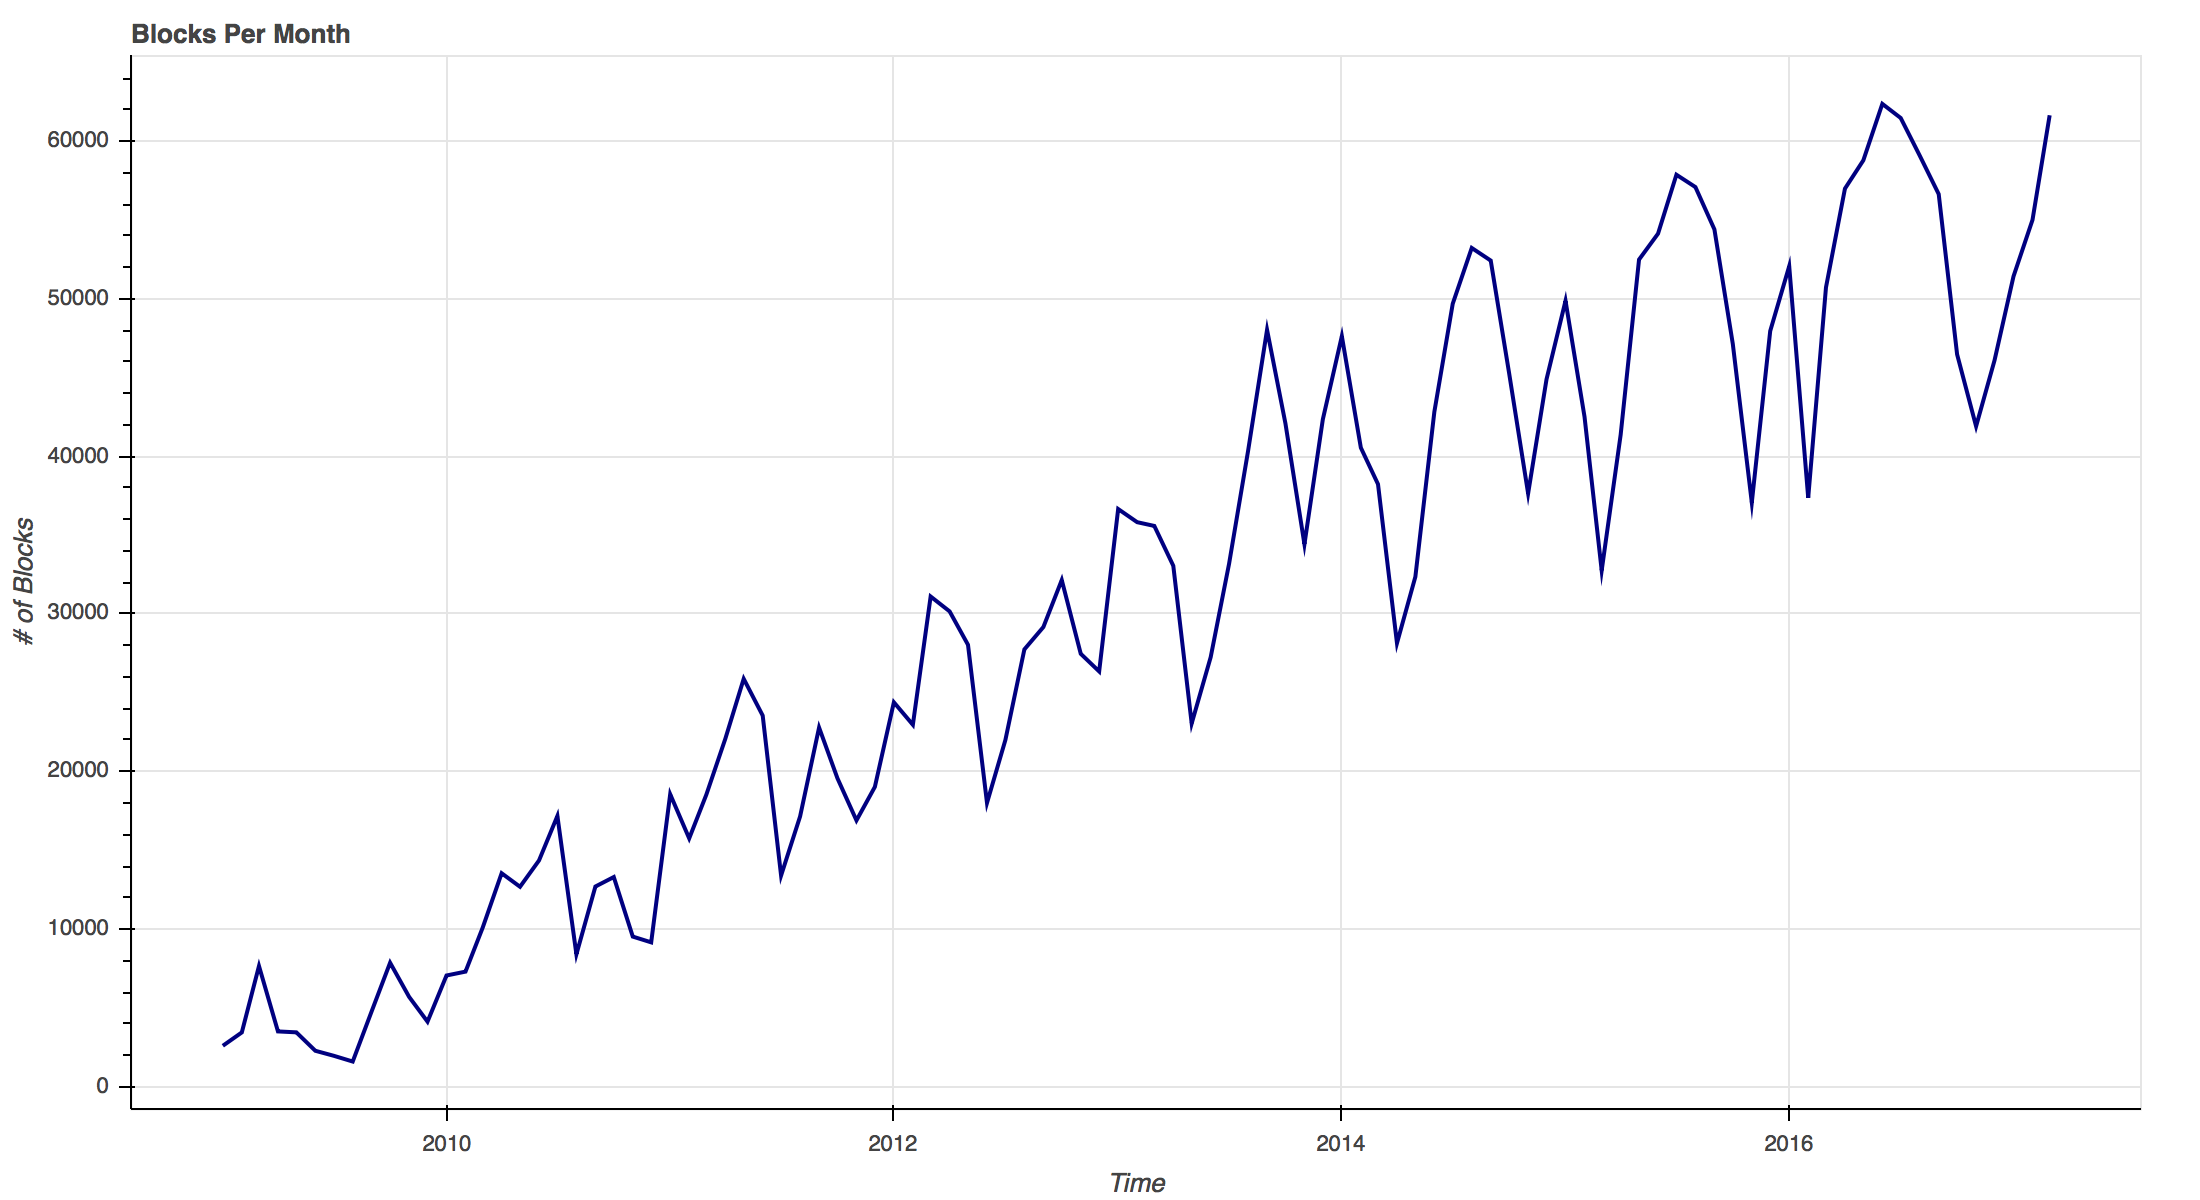
\includegraphics[width=9cm, height=5cm]{data/output/general/monthly_block_activity.png}
\end{figure}

\subsubsection{Transactions Per Month}
\begin{figure}[!ht]
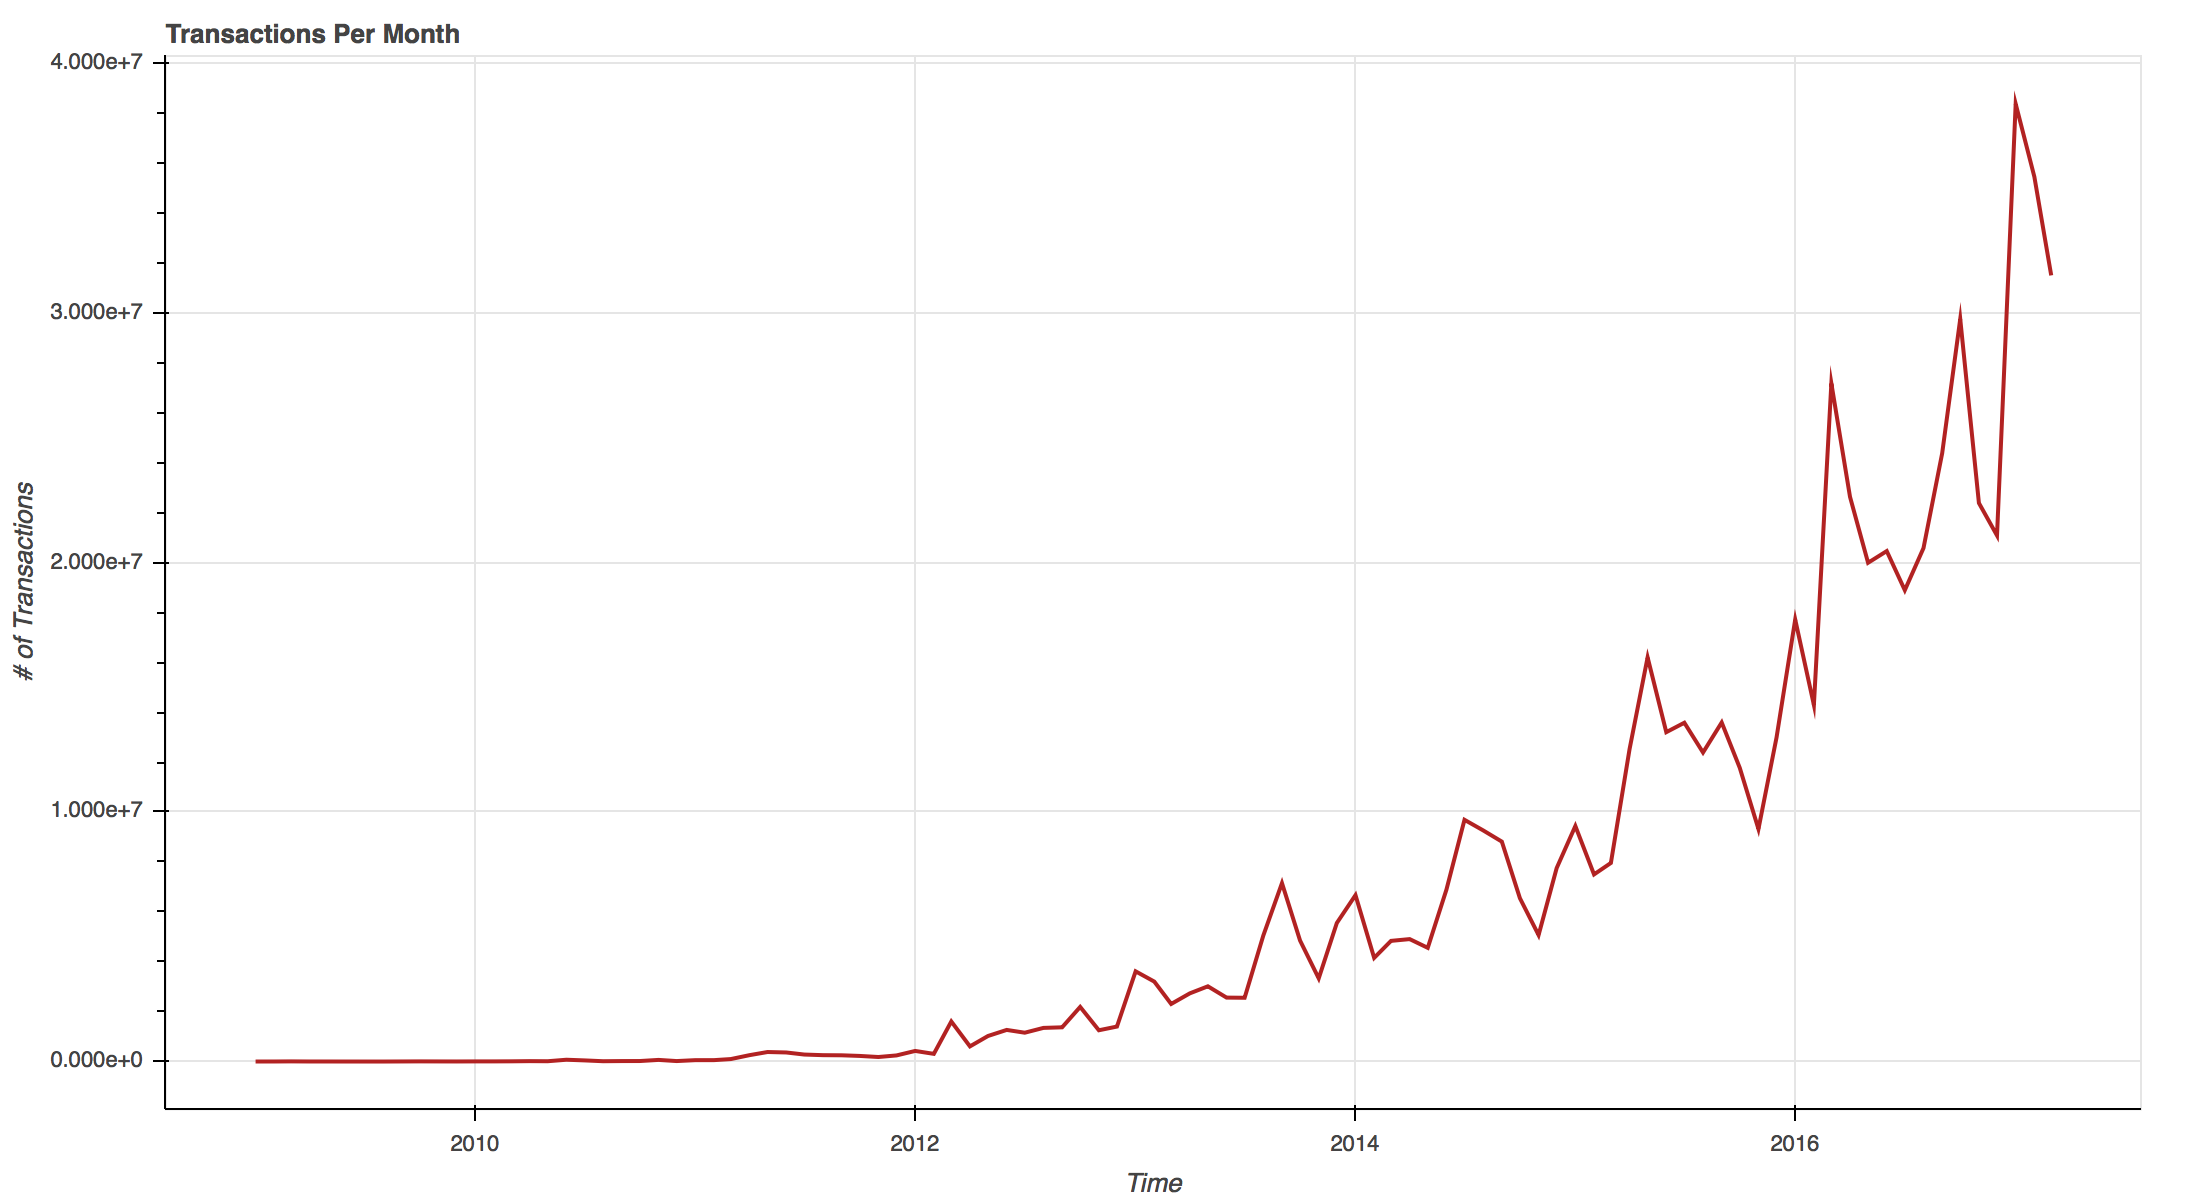
\includegraphics[width=9cm, height=5cm]{data/output/general/monthly_transaction_activity.png}
\end{figure}

\subsubsection{Monthly Transaction Volume}
\begin{figure}[!ht]
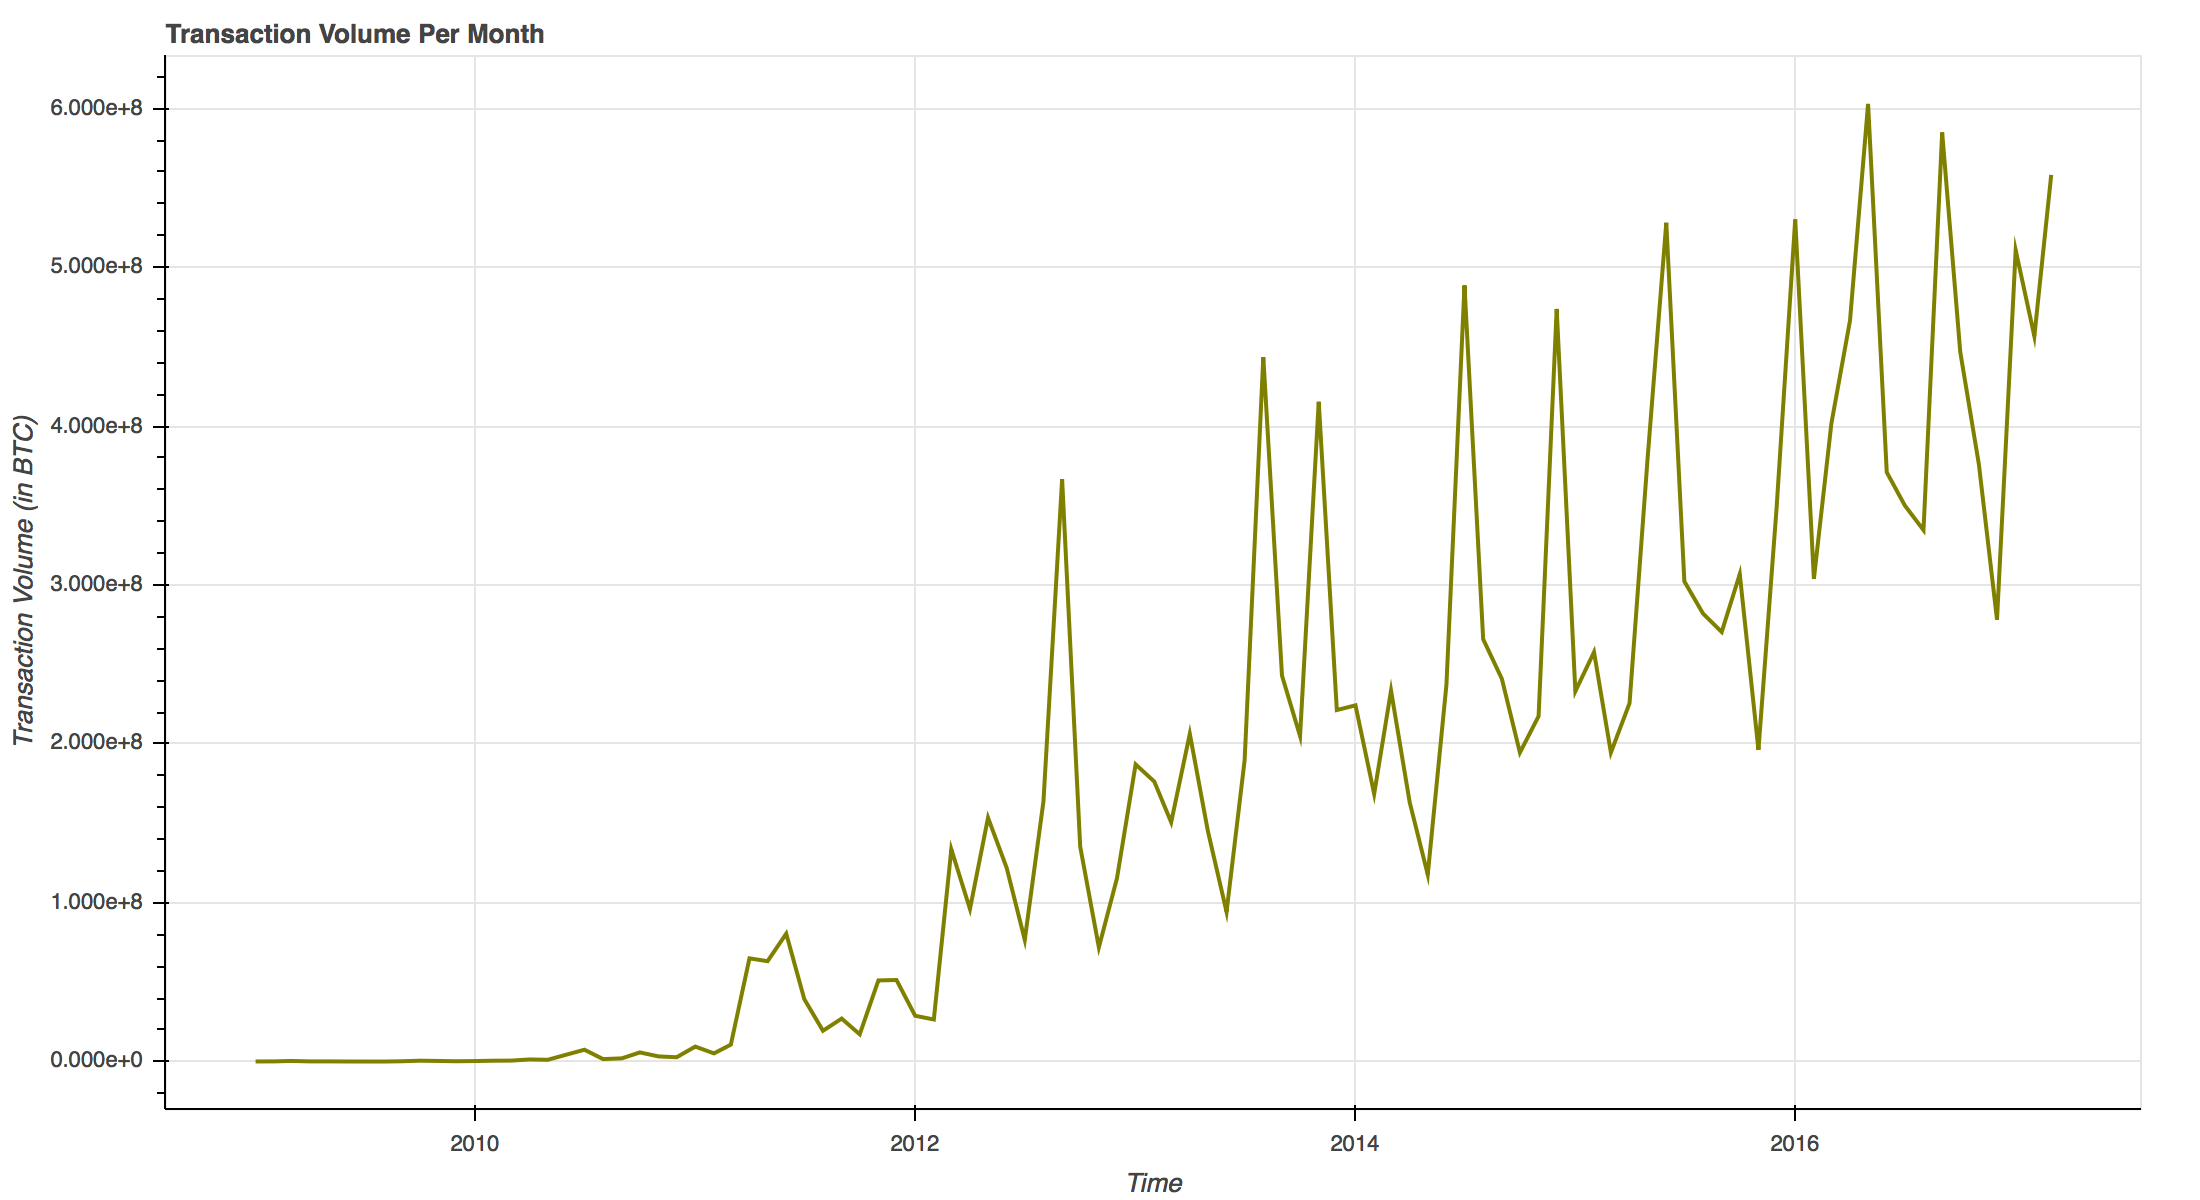
\includegraphics[width=9cm, height=5cm]{data/output/general/monthly_transaction_volume.png}
\end{figure}

\subsection{Address Growth}

The exact results from running this analysis can be seen \href{https://github.com/nishilshah17/idsi_bitcoin/blob/d2f1e0257ff684e99356de052eed1c6868ffe82f/data/output/new_addresses/new_addresses.txt}{here}. In the following graph, we have omitted results from April 2017 due to incomplete data from that month.

\begin{figure}[!ht]
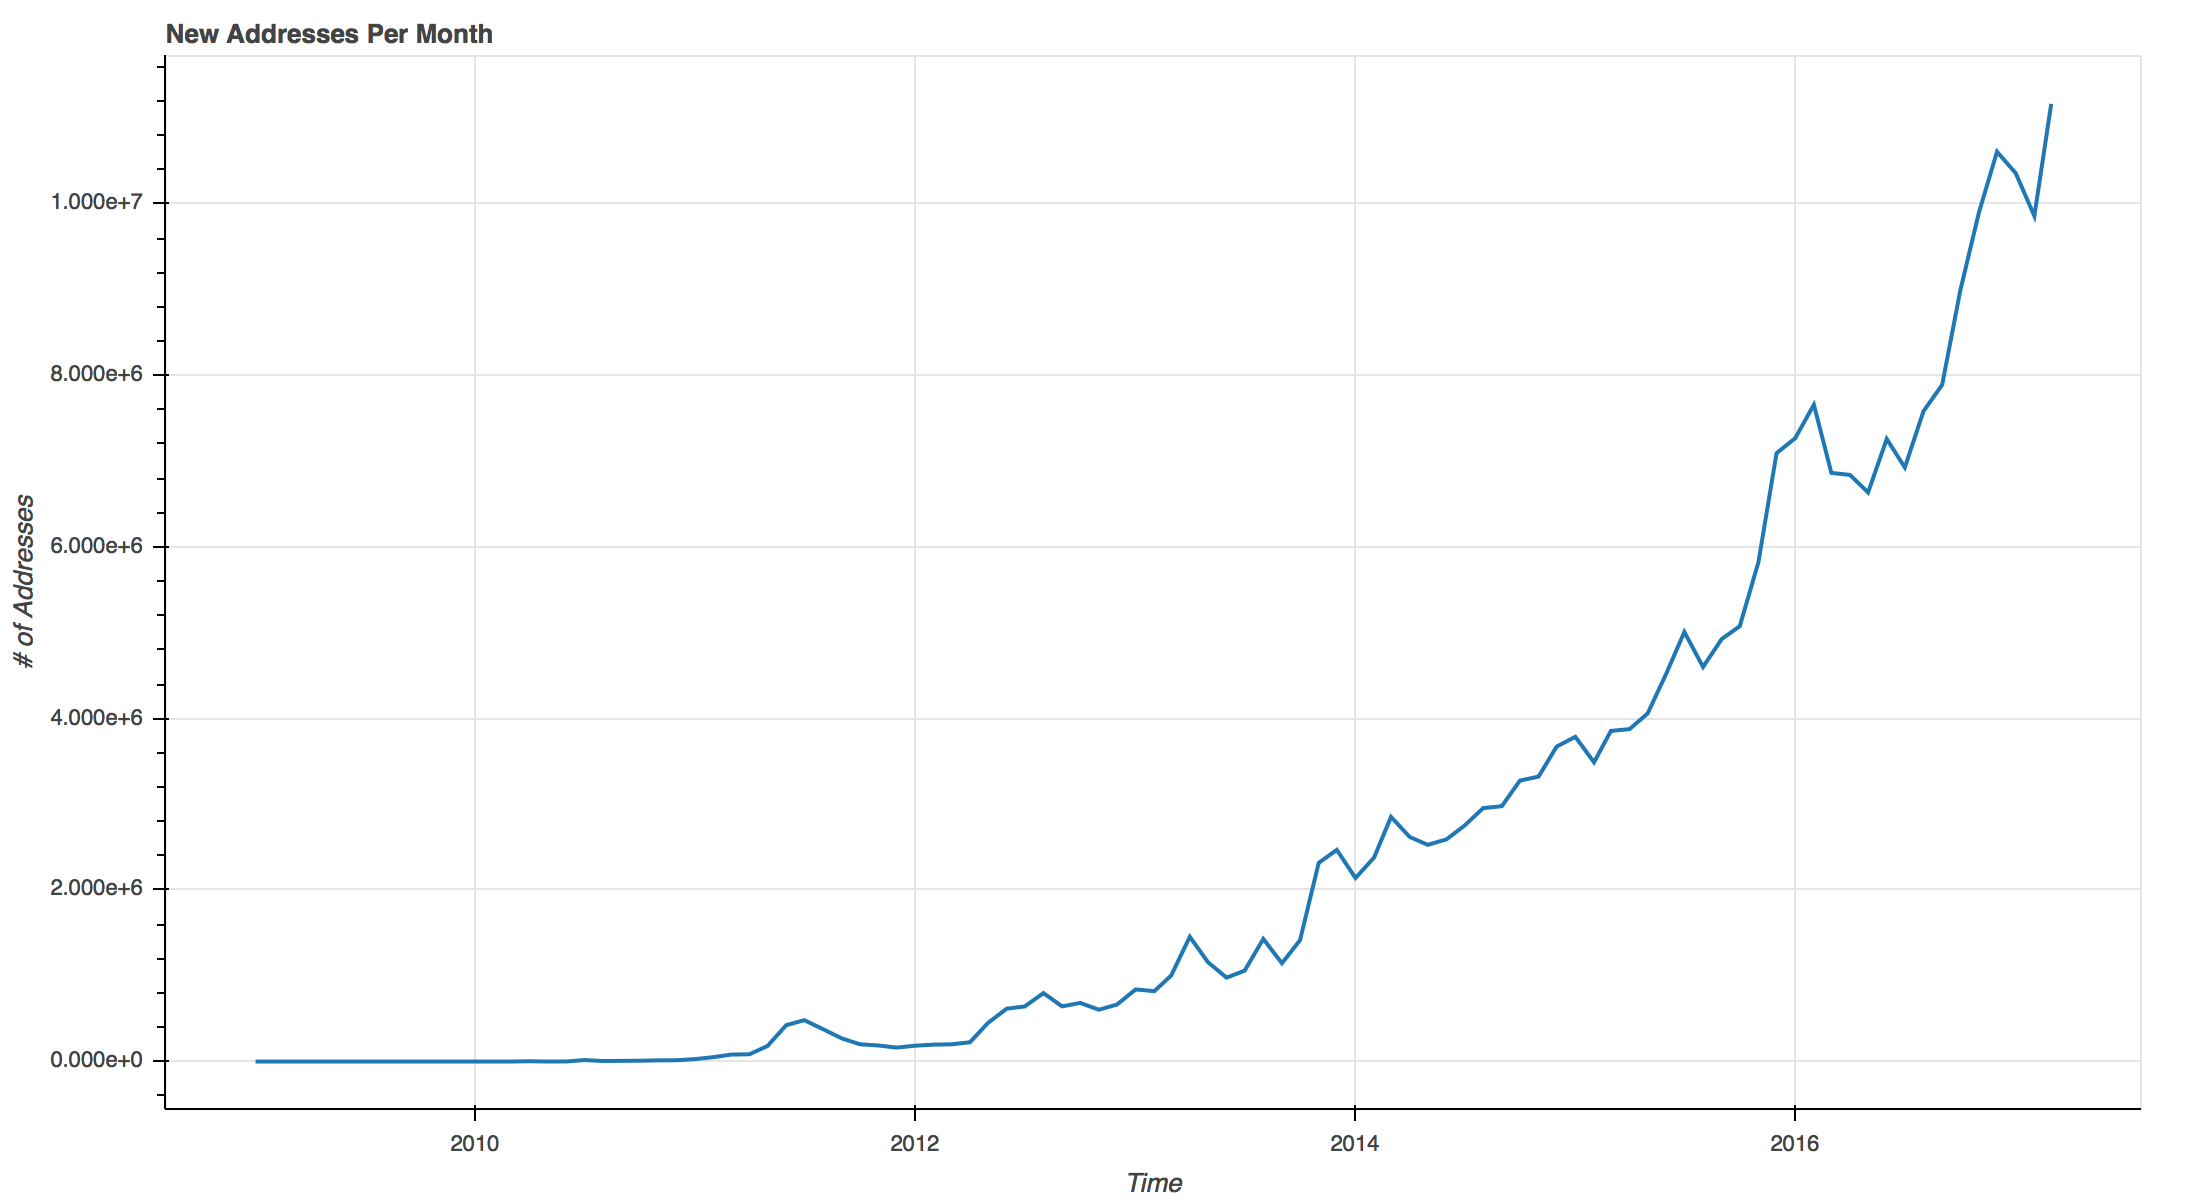
\includegraphics[width=9cm, height=5cm]{data/output/new_addresses/new_addresses.png}
\end{figure}

There is an obvious rapid and increasing growth in the number of new addresses used per month.

\subsection{Address Reuse}

/* LAST TODO */

\section{Other Applications}
This technical report provides just a brief introduction to the type of analysis that can be done on the Bitcoin blockchain. There are endless opportunities with this kind of financial data that we hope to explore and see in the future. For instance, we can attempt to identify entities/wallets from input and output addresses. This can lead to many conclusions such as how many Bitcoin the average person has and which wallets control the biggest share of the market. It would also be useful to look at patterns between certain transaction activity to Bitcoin/USD exchange price movements. A more complicated project could involve the classification of suspicious activity.


Additionally, we are not just limited to Bitcoin transaction data. There are numerous cryptocurrencies gaining popularity, most (if not all) of which operate using a similar decentralized ledger. All that is needed to expand this project to other blockchains is different methods of parsing the raw binary data.

\section{Conclusion}
In this technical report, we downloaded and performed an analysis on the full Bitcoin blockchain from the currency's inception until April 11, 2017. We discovered an upward trend in new addresses used per month, supporting an increase in Bitcoin adoption. We also looked into the reuse of addresses, which provides many insights. We found that XX percent of addresses are only used once and that addresses are reused an average of X.X times. This gives an estimate of how long people hold onto Bitcoin before spending it.

We have also seen the procedures involved in processing a large real world dataset with big data technologies such as Hadoop and Spark. Bitcoin is the biggest and most popular virtual currency in the world today. Every day, hundreds of blocks are being added to the blockchain that we explored in this technical report. This technical report is just a glimpse into the amount of information stored in the blockchain. There is a vast potential for future big data applications in this area.
\end{document}
